% Set the author and title of the compiled pdf
\hypersetup{
  pdftitle = {\Title},
  pdfauthor = {\Author}
}


\section{Recap of COMP12111 \& COMP15111}

There material in both the {\it Fundamentals of Computer Architecture} and the
{\it Fundamentals of Computer Engineering} courses in the first year provides a
good base for the course this year. The following re-visits that material and
builds upon it.

\subsection{Datapath and Control}

From the point of view of the CPU all data is of a fixed size, the length of one
word. Each word is usually moved around the architecture of the computer in a
bit-parallel manner, that is to say that there are at least the same number of
wires in a bus between any two components in the system as there are bits in the
word.

The individual operations on each bit inside a word when the CPU performs an
operation on the whole word are usually identical. This results in a very
regular datapath with lots of duplicated (usually by as many times as the word
length) hardware logic.

Control logic is derived after the datapath has been conceived. It governs which
operation is performed at what time, and is different for each instruction in
the instruction set.

A typical example of control logic might be to control the enable pin on a
binary adder. The datapath will direct bits to the adder all the time, but the
control logic will determine if the result is sent forward.

\subsection{The MU0 Instruction Set Architecture}

The MU0 is a very simple 16 bit word architecture, and as a result, the
instruction set is also very simple. Each instruction can address one memory
location, and consists of four bits for the instruction (allowing sixteen
instructions to be coded) and twelve bits for the memory address as illustrated
in Figure~\ref{instruction}. Since we can only store twelve bits of memory
address in the instruction, and the architecture is very simple, the system has
$2^{12}$ words of memory, which is equivalent to \SI{8}{\kilo\byte}.

\begin{figure}[ht!]
  \centering
  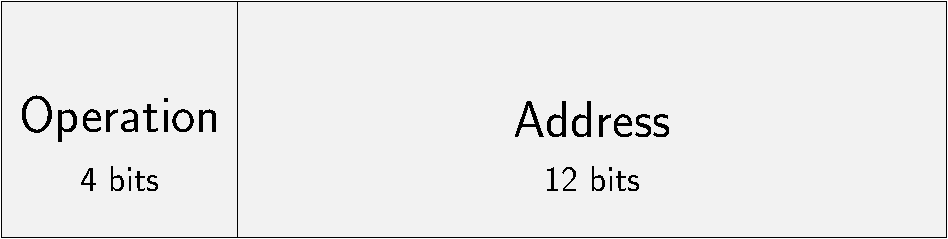
\includegraphics[width=90mm]{diagrams/instruction.pdf}
  \caption{A generic MU0 instruction}
  \label{instruction}
\end{figure}

The MU0 has two programmer visible registers, the Program Counter and the
Accumulator. The Program Counter stores the address in memory of the next
instruction to be executed, thus being twelve bits long. The Accumulator is
sixteen bits long, and stores the result of the last arithmetic operation.

The instructions that the MU0 understands are listed in
Table~\ref{instruction_set}.

\begin{table}[ht!]
  \centering
  \begin{tabular}{|c|c|c|}
    \hline
    {\bf Op Code} & {\bf Mnemonic} & {\bf Description}\\ \hline
    0 & LDA $[op]$ & $[op] \rightarrow Acc$\\ \hline
    1 & STO $[op]$ & $Acc \rightarrow [op]$\\ \hline
    2 & ADD $[op]$ & $Acc = Acc + [op]$\\ \hline
    3 & SUB $[op]$ & $Acc = Acc - [op]$\\ \hline
    4 & JMP $[op]$ & $PC = S$\\ \hline
    5 & JGE $[op]$ & If $Acc >= 0$ then $PC = S$\\ \hline
    6 & JNE $[op]$ & If $Acc \not= 0$ then $PC = S$\\ \hline
    7 & STP & Stop\\ \hline
  \end{tabular}
  \caption{The MU0 instruction set}
  \label{instruction_set}
\end{table}

\subsection{Maintaining Processor State}

If the execution cycle of the MU0 was somehow disrupted, say because of an
interrupt call, it would be handy to save the state of the processor before
switching to a different task (e.g. running the interrupt handler).

The way to do this is to save the registers in memory, doing the other task, and
then reloading them when it's time to resume execution of the program.

\subsection{The Fetch Execute Cycle}

The fetch-execute cycle describes how a CPU executes instructions. First, the
next instruction is fetched from memory (at the address pointed to by the PC),
then the instruction is executed. Since some instructions access memory (such as
load and store), and we can only do one memory access per clock cycle, one
fetch-execute cycle takes two clock cycles, one for fetching, and one for
execution.

\subsubsection{Fetching instructions}

Fetching is an operation that is the same for all instructions. First memory
addressed by the PC is read and stored into the Instruction Register (IR). This
is a 16 bit internal register that isn't visible to programmers. Once this has
occurred, the PC is incremented. This means that the RAM must be able to send a
word directly to the instruction register, so a datapath must be in place to
allow this.

\subsubsection{Executing instructions}

It is obvious that different instructions will have different paths of execution
within the processor, and will have different effects on components within the
system.

\paragraph{{\tt JMP}} In order to execute the {\tt JMP} instruction, the last
twelve bits are read from the instruction register and transferred over to the
PC. This means that there must be a datapath from the bottom twelve bits of the
IR to the PC.

\paragraph{{\tt STA}} When {\tt STA} is executed, the bottom twelve bits in the IR
are used direct the contents of the accumulator to a location in memory. To do
this, we need a datapath from the bottom twelve bits of the IR to the part of
the RAM that takes addresses, and from the PC to the part of the RAM that takes
data.

\paragraph{{\tt ADD}} To perform the {\tt ADD} instruction, we need to fetch the
bottom twelve bits of the IR and send it to the RAM. The result should be fed
into the adder along with the contents of the accumulator. The result of the
calculation should be sent to the accumulator. To do this, we need datapaths
from the accumulator to the ALU, the RAM to the ALU and finally from the ALU to
the accumulator.

\paragraph{Control Signals} whenever two separate components within the system
interact. For example, every time the CPU loads a word from the RAM, a control
signal must be sent to say `load', and every time the {\tt ADD} command it
executed, the ALU must be sent a control signal to say `add' as opposed to
subtract or shift.

\paragraph{Timing} Timing is very important when executing the instructions. If
the result of a load from RAM hasn't yet returned, but the control signal to the
ALU to add is sent, then the wrong result will almost certainly occur! In order
for everything to run smoothly, the critical path for each operation must be
worked out, and time allowed for signals to propagate through even the longest
critical path.

\subsubsection{Deriving the datapaths from the operation of instruction}

In order to produce a working processor, we need to look at all the instructions
that can be executed by the processor, and examine what datapaths and control
signals they require to work. Only when we have this information can we begin to
actually design the hardware on the CPU.

\marginpar{Note that data going to one destination can only go to one source, so
if you want multiple components to be able to send data to one other component,
then you must use a multiplexer with control signals in order to achieve this.}

\subsection{Control Signals}

The purpose of control signals is to make each component within the CPU function
as intended for each specific instruction. Control signals include:

\begin{itemize}
  \item Enable write for registers
  \item Enable write for memory
  \item Enable read for memory
  \item Multiplexer input select
  \item ALU actions (add, subtract, bypass)
\end{itemize}

Sometimes, one component (such as the ALU) may have control inputs that can be
represented by more than two states (add, bypass, subtract). If this is the
case, then multiple wires (a bus) is used to specify its action.

The first lab in the course shows the control signals sent for each instruction,
the solution for which is shown in Tables~\ref{lab:1:fetch} and
\ref{lab:1:execute}.

\begin{table}[!ht]
  \centering
    \begin{tabular}{|l|l|l|}\hline
    En\_IR  & 1 &(enable write to IR)\\ \hline
    En\_PC  & 0 &(enable write to PC)\\ \hline
    En\_ACC & X &(enable write to ACC)\\ \hline
    \hline
    byp & X &(ALU action: bypass)\\ \hline
    add & X &(ALU action: add)\\ \hline
    sub & X &(ALU action: subtract)\\ \hline
    \hline
    Ren & 1 &(RAM action: Read)\\ \hline
    Wen & 0 &(RAM action: Write)\\ \hline
    addr\_Mux& 1  &(RAM address = PC, otherwise IR.S)\\ \hline
  \end{tabular}
  \caption{The control signals in the MU0 fetch phase}
  \label{lab:1:fetch}
\end{table}

\begin{table}[!ht]
  \centering
  \begin{tabular}{|l|l|l|l|l|l|l|l|}\hline
      & lda & sta & add & sub & stp & jump  & no jump\\ \hline
    \hline
    En\_IR   & 0  & 0 & 0 & 0 & 0 & 0 & 0 \\ \hline
    En\_PC   & 0  & 0 & 0 & 0 & 0 & 1 & 0 \\ \hline
    En\_ACC  & 1  & 0 & 1 & 1 & 0 & 0 & 0 \\ \hline
    \hline
    byp      & 1  & X & 0 & 0 & X & X & X \\ \hline
    add      & 0  & X & 1 & 0 & X & X & X \\ \hline
    sub      & 0  & X & 0 & 1 & X & X & X \\ \hline
    \hline
    Ren      & 1  & 0 & 1 & 1 & 0 & 1 & 0 \\ \hline
    Wen      & 0  & 1 & 0 & 0 & 0 & 0 & 0 \\ \hline
    addr\_Mux& 0  & 0 & 0 & 0 & X & 0 & 1 \\ \hline
  \end{tabular}
  \caption{The control signals in the MU0 execute phase}
  \label{lab:1:execute}
\end{table}

\section{What does an Operating System do?}

The job of an operating system varies from system to system but on general, it
is responsible for managing the resources of the system (including dealing with
concurrency, security etc) and abstracting the implementation of the system from
the running programs (such as what exact components are being utilised).

\subsection{Processes}

A process is a program that is currently running on the system. It consists of a
Thread (a set of instructions to be executed) and address space (a set of memory
locations that can be accessed by the thread). In most systems, multi-threading
is used to allow each process own multiple threads, and therefore execute in
parallel.

\marginpar{Nearly all systems have many processes running at any one time, on a
Linux system, use {\tt htop} or {\tt ps aux} to see what processes are running.}

\subsection{Address Space}

\textit{Address space} (aka memory space) is a term used to speak about a
section of memory. This could be the whole memory available to the system, the
memory that a specific program has access to etc.

When a program starts, it assumes that it does so from memory address {\tt 0}.
On a single process system this is okay, however this presents a problem on
systems where multiple processes run concurrently, since no two processes can
share the same memory space.

Sometimes, operating systems may even running pause programs, move them out of
memory (onto secondary memory such as hard drive) and later on swap it back in
at a different place in memory.

In both cases, a technique called {\it Relocation} is used to make every running
program able to safely assume that it has sole use of memory.

In order to facilitate relocation, operating systems abstract away the
implementation of the hardware, and instead provide a virtual machine for each
program. This enables programs to behave as though they have the whole system
to themselves, and it also lets the operating system easily stop programs
interfering with each other (such as providing disjoint memory spaces for each
program).

\subsection{Modes of operation}

It is often necessary to prevent some programs from executing some operations,
such as manipulating memory, or allocating CPU time. In order to achieve this,
operating systems nearly always implement different `modes' of operation that
processes can run under. The two most common modes are \textit{user} and
\textit{system}.

All the processes owned by the operating system will run under system mode,
which is very permissive and lets programs perform operations with the
potential for misuse. Programs that the user might run are usually executing
under user mode. User mode is less permissive, and restricts certain
operations, yet the restricted operations aren't usually required for normal
programs.

\subsubsection{System calls}

If there was an eventuality where a program needed to perform privileged
operation that wasn't permitted under it's current mode, then it can use a
system call to achieve the same result. The premise is that the operating
system will provide a `gatekeeper' function that will perform the requested
operation, but only after the parameters have undergone checks to ensure that
the application isn't behaving badly. The execution of the user program will
(of course) pause while the system call is running.

Lots of functions in languages that you already know might just be wrappers
around system calls, albeit often with slightly more functionality. The course
notes make a good example; \texttt{fread} in C uses the \texttt{UNIX} system
call \texttt{read}.

\section{Engineering an Operating System}

Like a lot of things in Computer Science, operating systems can often be
conceptualised as being built up of several layers. As you inspect further and
further into the OS, looking deeper into each layer as you go, the level of
abstraction decreases.

The outermost layer could be seen to be the UI, which is obviously a very
abstracted way of thinking about a computer. The kernel is probably the lowest
layer, since the details of how the hardware is managed is, also fairly
obviously, a very low level of abstraction.

Different operating systems can contain a different number of layers of
abstraction so that they are best suited to their purpose. Some operating
systems will contain little more than a microkernel, which will have the bare
minimum of logic required to keep a computer running.

Some components of an operating system are monolithic, most notably the Linux
kernel. A monolithic component is easier to design (especially for a kernel)
since there is less inter-process communication to worry about, and trap falls
like race conditions can be more easily avoided when everything is running on
a single thread.

\marginpar{
  \begin{sloppypar}
    See this StackOverflow answer for an explanation (and follow the
    link to the Linus V Tanenbaum showdown on the topic):
    \texttt{http://stackoverflow.com/questions}
    \texttt{/1806585/why-is-linux-called}
    \texttt{-a-monolithic-kernel}
  \end{sloppypar}
}

I feel obliged to point out that monolithic, in this instance, refers to the
fact that the program is running under \textit{one} process that is in system
mode. It doesn't mean that the code is all in one big file, or even in one big
project, since many monolithic projects employ some degree of modularity in
the development process at least.

\subsection{Managing processes}

When operating systems were first developed, they usually ran one process at a
time. This was obviously limiting for the users, since only one person could do
stuff at a time. In light of this, timesharing was developed, which is a way for
the computer to be used by multiple users at once, even here, users would all
share one CPU and one PC though.

Now, processes execute within their own virtual CPU, while the real CPU switches
back and forth giving time to each task. This is good, since the order with
which the CPU gives it's time to processes can be used to effectively make some
processes run faster than others.

We have already learnt that a process is made up of a thread and some address
space, \marginpar{(Processes also have register values and external interfaces
too, but they're not as important)} but we've not been over how a process is
created. In order to do this, an existing process must create new child process.

Processes can be killed by themselves (with a variety of different exit codes),
by other processes (using something like the \texttt{kill}) command, or in some
systems, by the parent process terminating.

The lifecycle of a process, and the states it occupies can be represented in a
state machine like diagram, as shown in Figure~\ref{fig:proc-lifecycle}.

\begin{figure}[ht!]
  \centering
  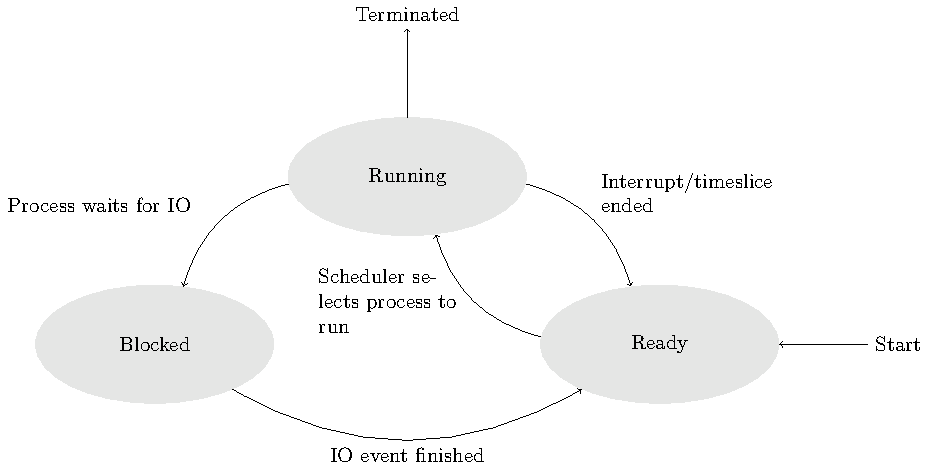
\includegraphics[width=\textwidth]{diagrams/process-lifecycle.pdf}
  \caption{The lifecycle of a process}
  \label{fig:proc-lifecycle}
\end{figure}

\subsubsection{Scheduling}

One particularly troublesome section of the lifecycle of a process is going from
the \textit{ready} state to the \textit{running} state (and vice versa). In
order to do this, a process to be resumed must be chosen from a pool of
processes waiting for CPU time, and the registers, IO operations etc must be
loaded and made ready.

In order to do this, a PCB (Process Control Block) table is maintained, which
contains all the necessary information for each process to be paused and
resumed. This includes (among other things):

\begin{itemize}
  \item Process ID
  \item Parent ID
  \item Saved registers
  \item Memory, IO management information
  \item CPU scheduling info
\end{itemize}

On some operating systems, timeslices are given to processes, where on others,
they are assigned to threads. Henceforth, processes can often be made more
efficient by using threads in order to maximise the use of their timeslice
(switching to non-blocked threads whenever there is a block).

In order to handle the complicated tasks of scheduling, operating systems have a
dedicated component as part of the process manager to do this. It's main job is
decide which process should run next on what core of the CPU, while minimising
the average wait and turnaround times for processes to execute.

Processes alternate between CPU (expensive computation) and IO (blocked on IO)
bursts. Processes that have long CPU bursts are said to be CPU bound, while
processes that use lots of IO are said to be IO bound. Processes can change
their characteristics while running (if a web browser is using lots of cached
content, it might be IO bound, but if it's rendering 4K video with JavaScript,
it's probably CPU bound).

Here are some scheduling algorithms:

\begin{description}
  \item \textbf{First Come First Serve (FCFS)}\\
    This is when processes get all of the CPU time until they are finished, or
    they block. It's easy to implement, since all you need is a queue of
    processes:

    \begin{figure}[ht!]
      \centering
      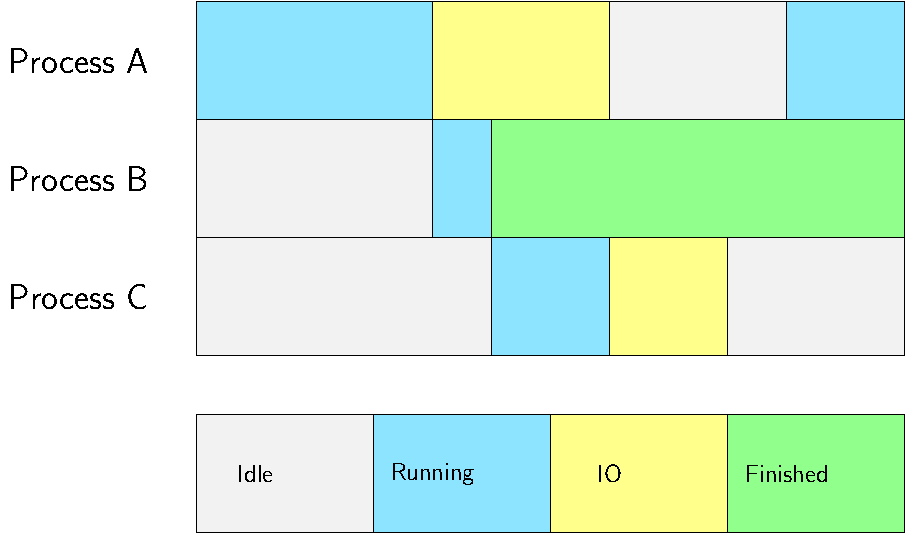
\includegraphics[width=90mm]{diagrams/fcfs.pdf}
      \caption{What an FCFS implementation might behave like}
      \label{fcfs}
    \end{figure}

    FCFS is a \textbf{non-preemptive} algorithm, since processes are allowed to
    run until they finish with the CPU and start doing IO stuff, or exit.

    \marginpar{`Time slice' is also known as `Time Quantum' and it's length is
    very important. Smaller time slices are affected greater by the time it
    takes to perform a context switch. The best solution is to try and decrease
    the cost of context switching and increase the time slice length a little
    (though not too much, otherwise you end up with psudo-FCFS)}

  \item \textbf{Round Robin}\\
    The round robin algorithm is a \textbf{preemptive} algorithm. Each process
    is given a time slice when it starts processing on the CPU, and if it hasn't
    finished by the end of it's time slice, then the CPU is given to another
    process. It's still a very simple algorithm, and it's much more efficient
    than FCFS.

    \begin{figure}[ht!]
      \centering
      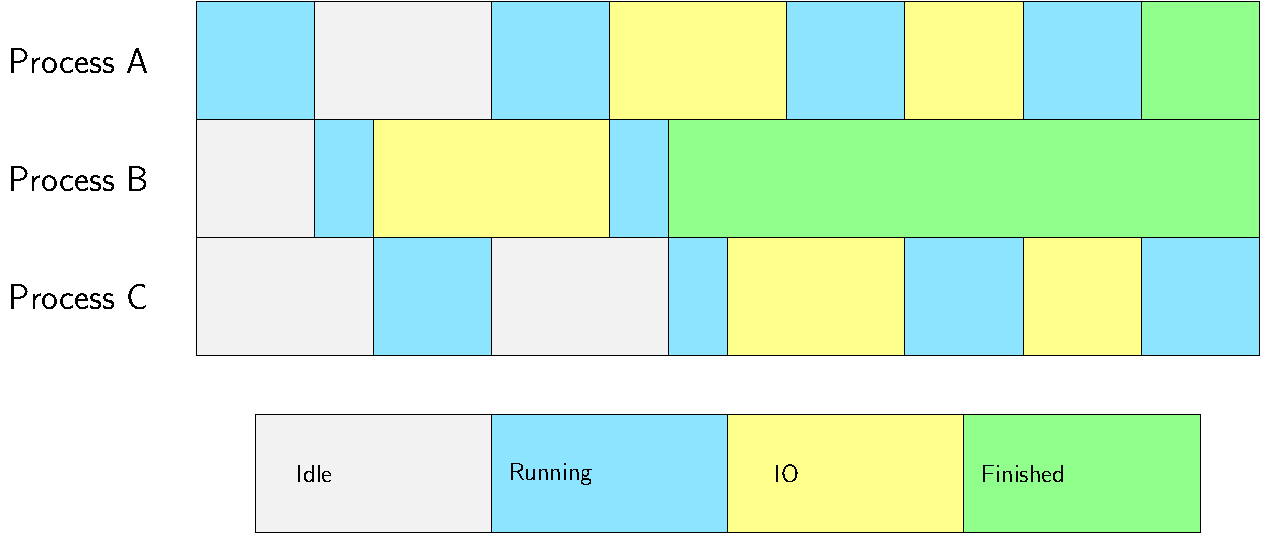
\includegraphics[width=90mm]{diagrams/roundrobin.pdf}
      \caption{What a Round Robin implementation might behave like}
      \label{roundrobin}
    \end{figure}

  \item \textbf{Shortest job first}\\
    We could just run whichever process will have the shortest CPU burst first.
    The problem with this one, is it can be hard to tell how long processes will
    use the CPU for. If we can pull this off though, the average turnaround time
    and wait time are very low. This would be a \textbf{non-preemptive}
    approach, since when a process starts to run, it is left running until it
    finishes it's CPU burst.

    You can also \textbf{make SJF preemptive}. In order to do this, when a new
    process is added to the queue, if it has a lower CPU burst than the
    remaining time on the currently running process, then context switch and run
    the new one first. This is called \textbf{STRF} (Shortest Time Remaining
    First).

    One problem with SJF, is that if a process has a very long CPU burst, then
    it may be starved of CPU time by the scheduler, since other processes, with
    a smaller initial burst will be allowed in first.

  \item \textbf{Priority Queue}\\
    We could have multiple queues, each with a different priority. Processes in
    higher priority queues could have longer time slices, or could finish all
    their CPU bursts before allowing other processes to start with theirs. We
    could still end up starving low priority processes using (particularly) the
    latter method, however, if we had the option to \textit{dynamically move
    processes between queues}, then we could solve this problem too.

    \marginpar{Can you work out the actual amount of CPU/IO/idle that the
    processes have? It's in the \LaTeX~source if you want to find out!}

    \begin{figure}[ht!]
      \centering
      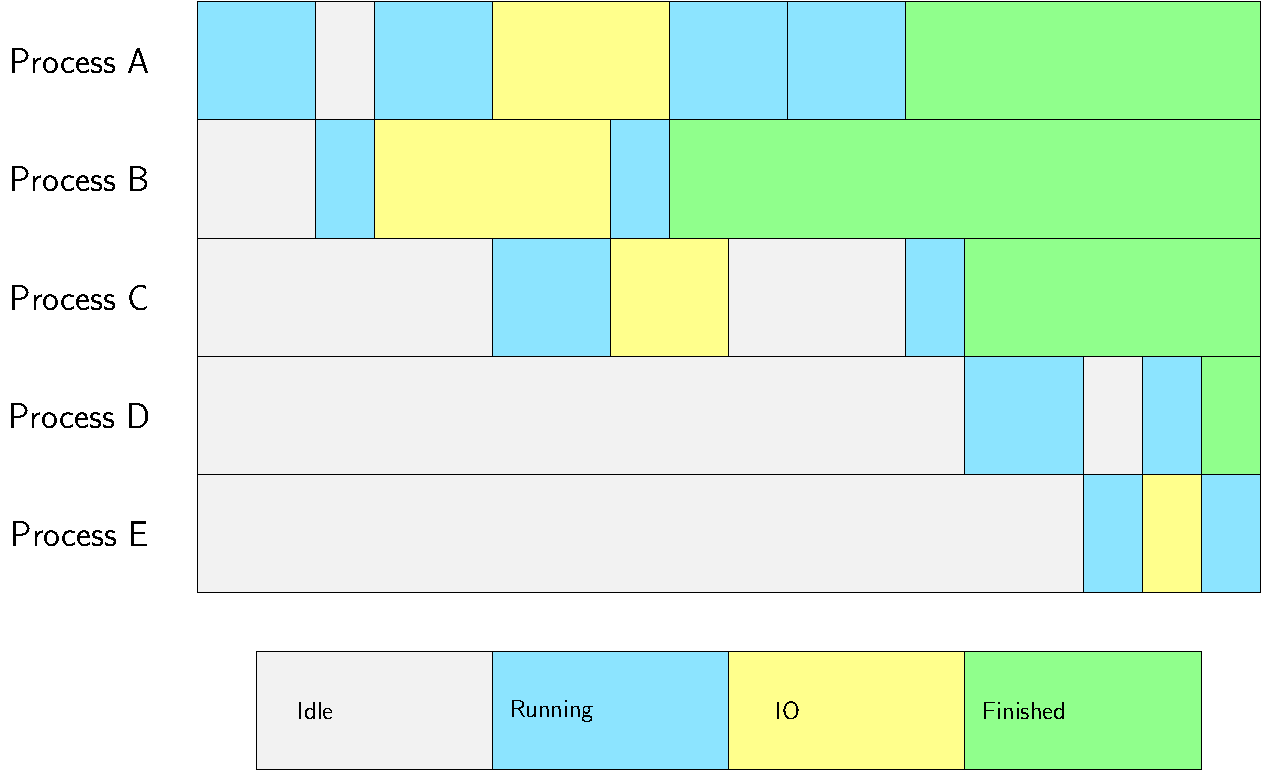
\includegraphics[width=90mm]{diagrams/priority.pdf}
      \caption{If process A and B were in the high priority queue, process C was
      in normal priority, while D and E were in low priority, the scheduler may
      behave like this.}
      \label{priority}
    \end{figure}

    Dynamically changing which queue processes are in sounds hard, but it's not
    too bad. Every time a process uses up all of it's timeslice, then move it
    down a queue, every time it finishes it's CPU burst before it's timeslice
    expires, move it up a queue. In this manner, IO bound applications will tend
    to execute faster, and there will be less idle time. \marginpar{This isn't
    really a good thing, since your IO programs (such as a backup utility), may
    not be the ones you want to run the fastest.}

    In earlier versions of Linux\footnote{
      If you're ahead of schedule with your revision, take a look at:
      \begin{itemize}
        \item \url{http://en.wikipedia.org/wiki/O(n)_scheduler}
        \item \url{http://en.wikipedia.org/wiki/O(1)_scheduler}
        \item \url{http://en.wikipedia.org/wiki/Completely_Fair_Scheduler}
      \end{itemize}
    }, there were three queues, but each used a
    different strategy; the highest priority queue was FIFO, the next queue used
    a round robin technique and the lowest priority queue used a method where
    the timeslice differs based on the process priority.

    The low priority queue is most interesting; each process has a quantum
    associated with it, which is reduced by one for each clock tick it has on
    the CPU. The timeslice it gets the process priority plus the remaining
    quantum divided by two. When all of the processes in the queue run out of
    quantums, then the quantum of all the processes in the queue is recomputed.

    Unfortunately, the old Linux way of scheduling didn't scale well, since it
    had an $O(n)$ runtime, so when you started up a lot of processes, the
    algorithm's performance would degrade. Now, Linux only uses algorithms with
    a $O(1)$ runtime, so that the number of processes doesn't impact on the CPU
    speed.

\end{description}

The above algorithms are targeted at desktop PC's, and `normal' operating
systems, but for applications that are a little different, such as real time
systems, then different algorithms are used (maybe one that picks the process
with a short deadline for computation, or the smallest deadline - completion
time).

\subsubsection{Context switching}

A context switch occurs whenever the CPU pauses execution for one process and
resumes it for another. It's sometimes and expensive operation, and depending on
the processor, can take anywhere from one micro-second to one nano-second.

\marginpar{It is important to remember that there are plenty of things that do
need to be included in the context switch when two threads of the same process
are swapping, including registers (including the PC), and the stack.}

It is important to realise that not all context switches are equal even on the
same machine. If the processor is switching between two threads of the same
process, it won't have to switch in most of the information about memory, since
the threads will use the same memory space. Because of this, the memory cache
might also be more efficient due to locality of reference.

\section{Synchronisation}

When two threads or processes haves access to the same data, there is a danger
that they could interfere with each other by using the data as a medium. This
issue is especially acute when there are two threads in the same process, since
they occupy the same memory space.

\textbf{Race conditions} can often occur as a result of shared access to data,
and when synchronisation isn't (properly) used to regulate execution. A race
condition is when one or more processes/threads execute in parallel, but the
outcome depends on which finishes (or gets to a critical section \marginpar{A
critical section is a block of code that uses data that is shared between
threads, consequently, only one thread should be `in' the critical section at
once.}) first. Since a thread is not guaranteed to always run at the same speed
(due to clock frequencies changing, hardware being busy etc), race conditions
are unpredictable, and are often hard to debug.

Data inconsistency can occur when threads are executing in parallel, but they
have different values for what should be the same data. This can occur when two
or more threads try and update (or read from) a variable at once. Although
reading and writing to a variable is often written as one instruction in most
reasonably high level programming languages, further down the software stack, it
could comprise of many CPU instructions If these were to interleave, then strange
things could happen.

For example, if I had one thread adding 10 to an integer (initialised to 0), and
another adding 6 this could happen:

\begin{lstlisting}
  Thread A: Read variable 
  Thread B: Read variable 
  Thread A: Add 10        
  Thread B: Add 6         
  Thread A: Write variable
  Thread B: Write variable
\end{lstlisting}

Now the value of the variable will be 6, since Thread A's write has been
overwritten by Thread B.

The solution to this, is to have only one thread in a critical section at once
(writing to the variable would be considered a critical section in this
instance). This idea is called \textbf{Mutual Exclusion}, since only one thread
can be active at a time. It is often achieved in the form of a mutex lock, which
a thread will occupy when it enters a critical section, and release when it
exits.

\subsection{Semaphores}

The famous computer scientist Dijkstra formulated a lightweight way to ensure
that only a specific number of processes would enter the critical section at any
one time, using only one integer variable.

If a process wanted to enter it's critical section, it would wait until the
Semaphore variable (\texttt{S}) was greater than zero. When it was, then the
process would decrement \texttt{S} and then enter it's critical section. When it
leaves it's critical section, it will increment \texttt{S} to indicate that the
`space' is free. See Listing~\ref{lst:semaphore} for an implementation.

\marginpar{There are numerous errors in Listing~\ref{lst:semaphore} (although
it's fine as an example), it wouldn't work very well in production, can you
spot them?}

\begin{lstlisting}[language=Java, label=lst:semaphore, caption={A Java
                   implementation of a Semaphore}]
  public abstract class Semaphore {
    private int S = 0;

    public Semaphore(int numThreads) {
      S = numThreads;
    }

    // P = Procure the critical section
    public synchronised void P() {
      while(S <= 0);
      S--;
    }

    // V = Vacate the critical section
    public synchronised void V() {
      S++;
    }
  }
\end{lstlisting}

Using an integer instead of a boolean is good, since it allows for a
configurable number of processes to be working concurrently in the critical
section, not just one. However, for most applications, only one thread can be in
the critical section at once for the aforementioned reasons.

Although it's easy to implement a semaphore that uses a while loop to wait until
another process is ready, this is very wasteful of CPU time (it's also known as
a busy-wait). A better way to do it is to halt execution of the thread
altogether until another semaphore space is ready. An example of this is given
in Listing~\ref{lst:semaphore-clever}.

\begin{lstlisting}[language=Java, label=lst:semaphore-clever, caption={A Java
                   implementation of a Semaphore that doesn't use busy loops}]
  public abstract class Semaphore {
    private int S = 0;

    public Semaphore(int numThreads) {
      S = numThreads;
    }

    // P = Procure the critical section
    public synchronised void P() {
      while(S <= 0) {
        try { wait(); }
        catch(InterruptedException e) { e.printStackTrace(); }
      }
      S--;
    }

    // V = Vacate the critical section
    public synchronised void V() {
      S++;
      if(S > 0) notifyAll();
    }
  }
\end{lstlisting}

\subsection{Deadlock}

Deadlock is when more than one process is waiting for something that can only be
provided by a process that is also in deadlock. It's a complicated thing for an
operating system to even detect, never mind solve.

\section{Java Threads}

For some reason, the University decides to teach us about Java threads in an
Operating Systems course, not in the Java course. Hmmm\dots.

The most basic way to run code concurrently in Java is probably to make a
subclass of \texttt{java.lang.Thread}, and call \texttt{start()}, or make your
class implement the \texttt{Runnable} interface.

\begin{lstlisting}[language=Java,caption=Extending the Thread class]
  class BitcoinMiner extends Thread {
    public void run() {
      // Mine many bitcoins...
    }
  }

  ...

  BitcoinMiner miner = new BitcoinMiner(...);
  miner.start();
\end{lstlisting}

\begin{lstlisting}[language=Java,caption=Using the runnable interface,
                   label=lst:doge]
  class DogecoinMiner implements Runnable {
    public void run() {
      // very mine..
      // such fun
    }
  }

  ...

  new Thread(new DogecoinMiner()).start();
\end{lstlisting}

Threads provide three notable methods:

\begin{description}
  \item \texttt{sleep(millis)}\\
    Sleeps the thread for an amount of milliseconds. Basically, it says
    \textit{I'm done with my timeslice, and please don't give me another one for
    at least n milliseconds.}
  \item \texttt{wait()}\\
    Stop executing the thread until somebody calls \texttt{notify()}.
    \textit{I'm done with my timeslice. Don't give me another timeslice until
    someone calls notify().}
  \item \texttt{notify()}\\
    Wakes up one thread that is sleeping.
  \item \texttt{notifyAll()}\\
    Wakes up \textit{all} the threads that are sleeping.
\end{description}

\subsection{The \texttt{synchronized} keyword}

In Java, every object comes with it's very own mutually exclusive lock. When the
object is locked, threads other than the one that locked the object cannot use
it until the object is unlocked by that thread, and therefore only one thread
can hold the lock at any one time.

Methods can also be made to come with a built in lock, in order to do so, you
must declare them as \texttt{synchronized}. The lock must be obtained before the
method will start (even though it may have been called).

Locks are automatically obtained and relinquished (kind of), so synchronization
is important to get right when you're writing your methods and objects, but less
so when you're using them.

You can, in fact, synchronize any block of code, by wrapping it in a
\texttt{synchronized(expression){...}} block. The expression is an object whose
lock will be held while the block of code between the curly brackets is
executed.

You can see in Listing~\ref{lst:semaphore-clever}, I've used a \texttt{while}
loop to make the thread wait. This is because we might not always obtain the
lock on the first go. Likewise, I also used \texttt{notifyAll()} in case a
thread doesn't wake up properly or doesn't receive the wakeup.

\section{Memory Management}

Random Access Memory (RAM) is one of the most important resources for a
computer, and making efficient and safe use of it is important for a well
running Operating System.

\subsection{Uniprogramming}

In a Von Neumann architecture RAM is used to store both programs and data. If an
older OS wanted to run a program, it would load the program into RAM, move the
PC to the start of the program in RAM and start executing. This method of
executing programs is called \textbf{Uniprogramming}. It seems rather simple,
but it has the following drawbacks:

\begin{itemize}
	\item We don't know in advance what the base address (the start address) of
	the program will be. This could be problematic if the program has hardcoded
	addresses in it.
	\item If the memory (synonymous with RAM) is too small, then we can't
	execute the program.
\end{itemize}

\subsection{Multiprogramming}

Multiprogramming breaks the main memory down into fixed partitions (also called
\textit{frames}) that can each hold (sections) of a program. This allows
multiple programs to be loaded (and executed) at once.

\begin{center}
	\begin{drawstack}
		\cell{OS}	         \cellptr{\texttt{0xFFFF}}
		\cell{Program x}     \cellptr{\texttt{0xC000}}
		\cell{Program z}     \cellptr{\texttt{0x8000}}
		\cell{Program y}     \cellptr{\texttt{0x4000}}
		\cell{Program x Data}\cellptr{\texttt{0x0000}}
	\end{drawstack}
\end{center}

The method of assigning programs frames allows programs to be swapped in and out
of memory based on when they are needed. This strategy of partitioning the main
memory has it's drawbacks though; if a program can write to any part of the RAM,
then malicious or badly made programs could overwrite parts of other programs,
which could change what the program does, or change the data it's using.

We still haven't solved the problem that some programs may have hardcoded memory
addresses in them. The solution to this is to have a `loader' which changes all
the memory addresses in the program to accommodate the fact that the program
isn't really running from \texttt{0x0000}. It does this by adding $n$ to the
memory addresses, where $n$ is the `real' base address of the program.

\marginpar{Why don't we need to worry about malicious programs editing data in
frames with lower memory addresses?}

In order to stop programs from accessing memory outside their frame, a limit can
be implemented when the loader edits the memory addresses, which ensures that
the program cannot see or mutate data outside it's frame. The limit is
initialised to be the length in bytes of the program.

\marginpar{The MMU (Memory Management Unit) is a piece of hardware that sits
in between the processor and the main memory.}

All of the address translation goes on in the \textbf{MMU}, which is convenient,
since we can easily implement logic such as this in fast hardware, as shown in
Figure~\ref{mmu-translate}.

\begin{figure}[ht!]
  \centering
  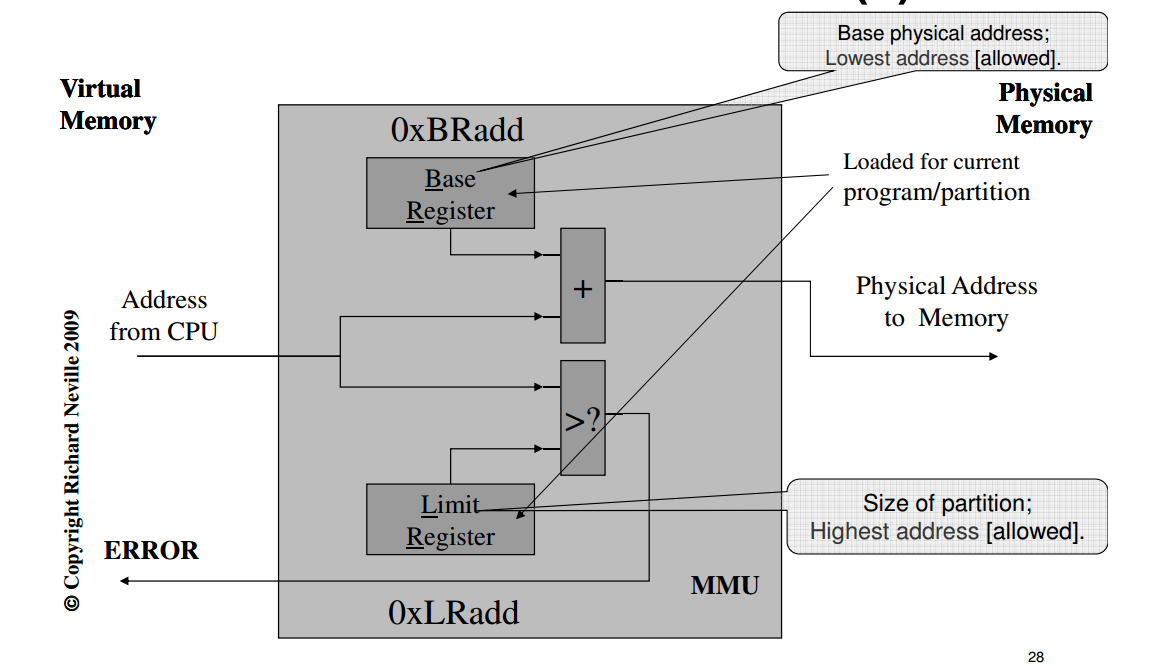
\includegraphics[width=\textwidth]{images/mmu-loader.jpg}
  \caption{How the MMU could translate addresses for execution. This diagram is
  taken from the course notes, \textcopyright Richard Neville 2009}
  \label{mmu-translate}
\end{figure}

Since programs that use hardcoded addresses in memory aren't \textit{actually}
using those addresses, they are referred to as `\textbf{virtual addresses}'.
When a virtual address has been translated into the actual address and put into
memory, it is called a `\textbf{physical address}'.

\subsubsection{Swapping}

I've alluded to the fact that a computer could have more programs running than
are currently in memory, but this section makes it explicit. When there isn't
enough main memory to hold all of the running programs, some of them can be
transferred onto disk for a short time until they need to be executed again.

There are strategies for keeping the `right' programs in memory, and to mitigate
the delays that the IO brings. Variable sized partitions are also used to make
sure that as little space in the RAM is wasted as possible.

The memory can still get very fragmented though; programs allocate memory
dynamically, and so the required size of frames could be unknown\dots

\subsection{Virtual Memory}

Virtual memory is there in order to allow the processor to address a larger
range of address spaces (than there is in the physical memory), and to support
the operating system in managing processes.

The MMU uses a \texttt{page table} (which is maintained by the operating system)
that is used to translate between physical and logical addresses. The
translation must be \textit{very} fast since every read and write to the memory
will go through it.

There are two techniques used to implement virtual memory; \textit{paged}
virtual memory and \textit{segmented} virtual memory. Paged memory is split into
fixed sized chunks called, you guessed it, pages. Segmented memory is split into
chunks of a variable size. As you may have been able to tell from exploits into
programs like Windows Task Manager, paging is the most commonly used method of
implementing virtual memory.

\subsection{Virtual paged memory}

The number of pages used in the system is given by the formula:

\[
	\#pages = \frac{\text{Address Space (bits)}}{\text{Page size (bits)}}
\]

If you want to find how many page frames (each one is the same size as a page)
there are in the physical memory, then just substitute the Address Space in the
above equation for the size of the physical memory.

When using paged memory, the processor gives two numbers when it wants to access
a memory cell, the page number, and the offset. These numbers are usually
contiguously melded together into one long number, where the first $log_2(n)$
bits (where $n$ is the number of pages in the virtual memory, given by $2^x$,
where $x$ is the number of bits in a machine word) is the page number, and the
rest of the bits is the offset. This is depicted in Figure~\ref{memory-address}.

\begin{figure}[ht!]
  \centering
  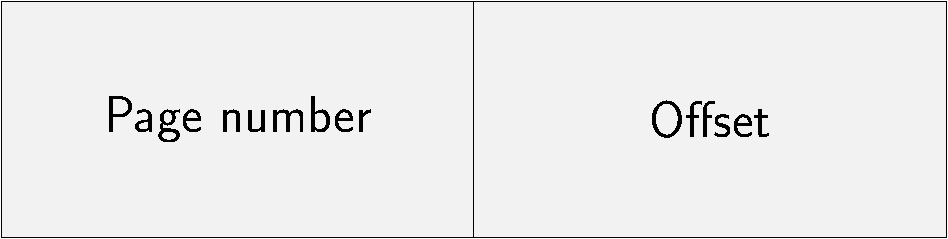
\includegraphics[width=90mm]{diagrams/memory-address.pdf}
  \caption{The format of an address to paged memory}
  \label{memory-address}
\end{figure}

When the MMU gets a paged address, it follows these steps:

\begin{enumerate}
	\item Look up the page number in the page table, see if the page is in the
		physical memory or not.
	\item If the page is in memory, generate a physical address (
		$(\text{page-size} \times \text{page-number}) + \text{offset}$), and
		request that from the RAM.
	\item If it's not, then abort the memory access, and the operating system
		will load the page into memory (this is a \textbf{page fault}).
\end{enumerate}

\marginpar{
	A \textbf{Page Fault} is when a page is on the backing store, but is needed
	by a process. If this happens:

	\begin{enumerate}
		\item The current processes is halted.
		\item The OS will load the page into physical memory.
		\item While the page is loading, other processes will have CPU time.
		\item Once the page has been loaded into RAM, the memory reference will
			be retried.
	\end{enumerate}
}

The page table contains one row for each page. The columns will include:

\begin{description}
	\item \textbf{Resident flag}\\
		If the page currently in virtual memory?
	\item \textbf{Used flag}\\
		Has the page been used?
	\item \textbf{Dirty flag}\\
		Has the page been written to while it's been in physical memory (so it
		needs to be copied back in full when it's put back onto the disk).
	\item \textbf{Physical address}\\
		The base address of the page in RAM.
	\item \textbf{Disk address}\\
		The base address of the page on backing store.
\end{description}

\subsubsection{Page replacement algorithms}

After a while (or not a while if you've not got much RAM), all of the page
frames will be occupied in memory. This means we need to swap one page for
another in the main memory next time we have a page fault. We need an algorithm
to determine which page to swap. The LRU (Last Recently Used) and FIFO (First In
First Out) algorithms are good for this.

If we make bad choices about which pages to reject from memory, then our
performance can seriously degrade. The following algorithms try and find the
best page to swap out whenever we've got a page fault on our hands. An ideal
solution is to find the page that will be used furthest in the future and swap
that one out, but since we don't know in advance what memory programs will want
to use (programs are dynamic), we can't do this.

\begin{description}
  \item \textbf{First In First Out (FIFO)}\\
    Identifies the oldest page in memory and gets rid of that. This is risky,
    since old pages can be critical pages (such as the operating system for
    example, that's going to be loaded into RAM pretty early on isn't it!).

  \item \textbf{Second Chance Algorithm (SCA)}\\
    This algorithm is similar to FIFO, except that the oldest page with the
    fewest number of accesses since the last pass of the algorithm is removed.
    It's implemented by keeping a count of page accesses, that is reset on every
    pass of the algorithm.

  \item \textbf{Last Recently Used (LRU)}\\
    The LRU algorithm works on the principle that if a page has been used
    recently, then it's probably going to be used again soon. The easiest
    implementation is to have a timestamp for every page (32/64 bit counter)
    that is updated whenever the page is accessed. This can be slow when
    implemented in software, so it's often added as a counter in the Translation
    Lookaside Buffer (TLB)\marginpar{The TLB is a cache that's used to improve
    the virtual address translation speed. Most PC's have one.}, which is
    expensive in terms of hardware, but is fast.

  \item \textbf{Not Recently Used (NRU)}\\
    The NRU algorithm is a dumb replacement for LRU. It keeps an extra bit
    called the `referenced bit' in the page table, that is set to $1$ when the
    page is referenced. When a page needs to be replaced, ones with their
    reference bit set to zero will be candidates. At fixed intervals, all of
    these bits will be reset to $0$ (so all pages don't get `recently used'
    eventually).
\end{description}

\subsubsection{Swapping pages}

If we do want to swap a page in physical memory, we first need to decide if we
are to write it back to the disk. This is done by inspecting the dirty bit in
the page table, and is called a \textbf{write-back}. An alternative strategy is
\textbf{write-through}, where you write to RAM and disk every time, (so you
don't need to copy the whole page on every swap), however, this is silly, since
you spend ages waiting for disk IO.

\subsection{Virtual segmented memory}

The idea behind segmented virtual memory is similar to that of paged virtual
memory, except that the segments (nearly synonymous with pages) are of a
variable size. The motivation behind segmentation is about supporting the system
as a whole by allowing multiple address spaces, rather than enabling us to
address a larger memory space (like it is with paging), though that is a side
effect of segmented memory too.

However, unlike a page, a segment is a variably sized block of virtual address
space, and each segment has attributes that define how it is used, these include
access rights (which users can use the segment), and usage rights (what
operations can be performed on the segment, read/write/execute). Also unlike
pages, programmers can actually \textit{segments}!

Really though, in most respects, paged and segmented memory is really quite
similar:

\begin{itemize}
  \item Both segmentation and paging ensures that programs don't interfere with
  each other by writing to (or   reading from) each others memory. This
  protects against malicious and badly   made programs; if a program could
  write to the OS's memory, then the OS could be taken over by a malicious
  program!

  \item Both act like a mini address space, starting from address 0, and ending
  at address $n$, where $n$ is the length of the page in bytes.

  \item The address of a segment is made up of a segment number and an offset,
  just like the address of a page is made up of a page number and offset.

  \item A table of segments/pages is kept by the OS that keeps informational
  about the segment/page. The only difference for segments is that an additional
  field for the segment size is added.
\end{itemize}

Figure~\ref{memoryMap} shows how pages and segments are mapped from number-
offset combinations onto actual address space locations.

\begin{figure}[H]
  \centering
  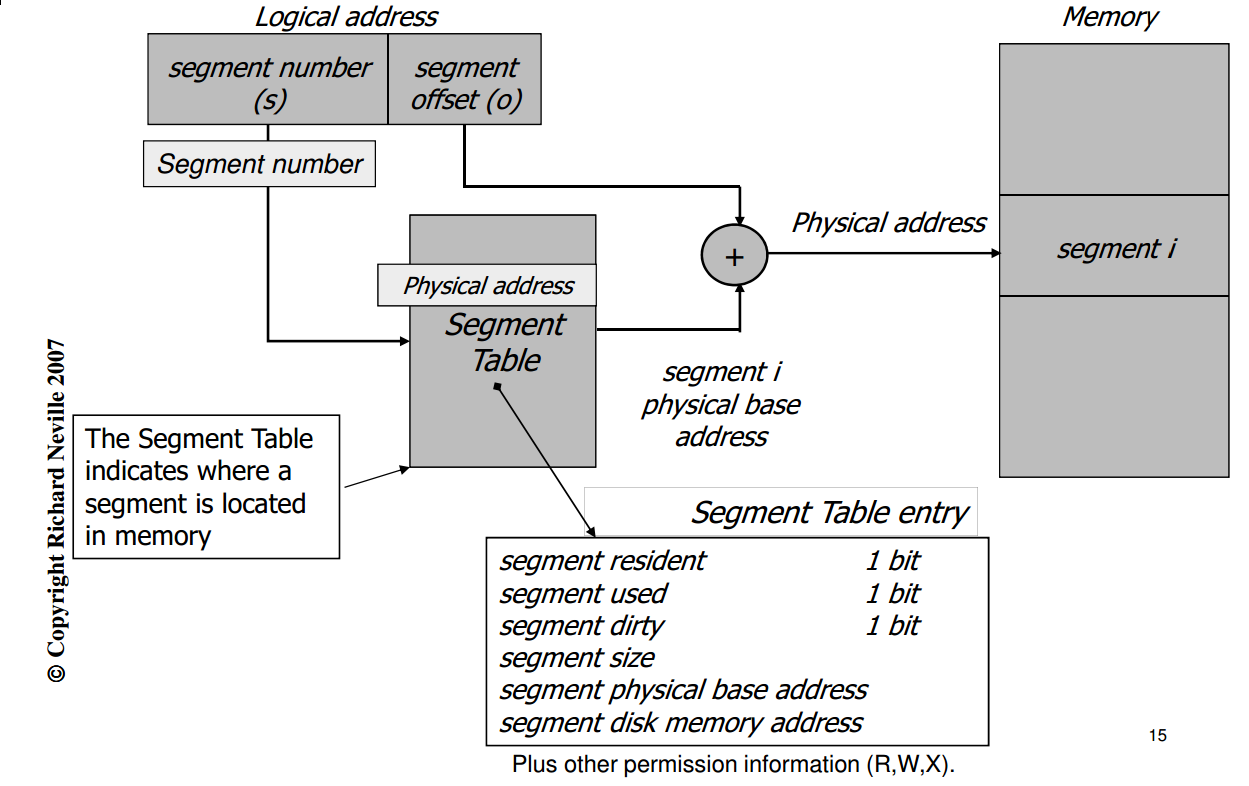
\includegraphics[width=90mm]{images/memoryMapping.png}
  \caption{Richard's diagram of \textbf{virtual address mapping} for segmented
  memory (it's really similar for paged memory too)}
  \label{memoryMap}
\end{figure}

A \textbf{segment fault} occurs if the OS tries to get a segment that is not in
memory. If this occurs, then the page must be loaded from the hard drive into
memory before it can be accessed. This isn't necessarily a \textit{bad} thing,
but it will take time to move the segment from the hard drive onto memory, and
potentially free up space in memory for it first.

The position of segments in memory is harder to manage than that of pages, since
segments come in different sizes. The OS needs to decide where to put segments
in the memory, and what to do with fragmented memory. Fragmentation of the
memory space builds up over time as segments of different sizes are moved
between main memory and the backing store. This is called \textbf{External
Fragmentation}.

The OS compacts fragmented memory by shuffling segments to fill the holes,
however, this is expensive since whole fragments must be copied (potentially
lots of data). Of course, it's better to avoid fragmentation in the first place?

When the OS is placing segments in memory, it can use algorithms such as best
fit (scan all the holes in the memory, and find the closest fit), or first fit
(shove the segment in the first hold that's big enough). The first tends to
produce lots of small holes (which is more efficient), while the second is
faster. All of these are a lot more intensive than the LRU and FIFO algorithms
we saw with paging.

The above points can make segments a lot less efficient than pages (especially
since some segments can be just a few bytes, which incurs a lot of overhead for
the amount of data being used), but the extra power that they give to
programmers makes them a good trade off.
